% =============================================================================
%  QUOKKAGUARD — paper 014 (Safe Medical-Device
%  Integration). House style derived from papers/_template.
% =============================================================================
\documentclass[11pt]{article}
\usepackage[utf8]{inputenc}
\usepackage[margin=1in]{geometry}
\usepackage{booktabs}
\usepackage{graphicx}
\usepackage{float}
\usepackage{afterpage}
\usepackage[section]{placeins}
\renewcommand{\topfraction}{0.9}
\renewcommand{\bottomfraction}{0.8}
\renewcommand{\textfraction}{0.08}
\renewcommand{\floatpagefraction}{0.75}
\setcounter{topnumber}{3}
\setcounter{bottomnumber}{2}
\setcounter{totalnumber}{5}
\usepackage{amsmath}
\usepackage{amssymb}
\usepackage{hyperref}
\usepackage{xcolor}
\usepackage{listings}
\definecolor{kwblue}{rgb}{0.10,0.20,0.65}
\definecolor{typepurple}{rgb}{0.50,0.15,0.55}
\definecolor{strred}{rgb}{0.62,0.12,0.12}
\definecolor{cmtgreen}{rgb}{0.20,0.45,0.20}
\lstdefinestyle{housespecyaml}{
  basicstyle=\ttfamily\footnotesize,
  backgroundcolor=\color{black!3},
  frame=single,
  framesep=5pt,
  rulecolor=\color{black!45},
  columns=fullflexible,
  breaklines=true,
  keepspaces=true,
  showstringspaces=false,
  alsoletter=_,
  commentstyle=\color{cmtgreen}\itshape,
  stringstyle=\color{strred},
  morecomment=[l]{\#},
  morestring=[b]",
  morestring=[b]',
  keywordstyle=\color{kwblue}\bfseries,
  keywords={device,risk_class,params,min,max,requires_confirm,interlocks,alarm_params,safe_state,version},
  keywordstyle=[2]\color{typepurple}\bfseries,
  keywords=[2]{life_sustaining,life_supporting,monitoring,allow,deny,clamp,escalate,revert_to_safe,freeze,handoff},
}
\lstdefinestyle{housespecyamlbare}{style=housespecyaml, frame=none,
  backgroundcolor=\color{white}, xleftmargin=0pt, framexleftmargin=0pt,
  aboveskip=1pt, belowskip=0pt}
\usepackage[most]{tcolorbox}
\tcbuselibrary{listings,skins}
\usepackage{tikz}
\usetikzlibrary{positioning,shapes.geometric,arrows.meta,calc,fit,backgrounds,shadows}
\definecolor{cardindigo}{HTML}{4F46E5}
\definecolor{slate}{HTML}{475569}
\definecolor{amber}{HTML}{D97706}
\definecolor{cardblue}{HTML}{1D4ED8}
\definecolor{cardpurple}{HTML}{6D28D9}
\definecolor{cardteal}{HTML}{0F766E}
\tcbset{
  cardcol/.store in=\cardcol, cardcol=cardblue,
  policycard/.style={
    enhanced, breakable=false, arc=3pt, boxrule=0.7pt, top=3pt, bottom=3pt,
    left=7pt, right=7pt, boxsep=1pt, coltitle=white,
    colframe=\cardcol!60!black, colback=white, colbacktitle=\cardcol,
    fonttitle=\bfseries\small, drop fuzzy shadow=black!25,
  },
}
\usepackage{url}
\usepackage{multirow}
\usepackage{array}
\usepackage{ragged2e}
\newcolumntype{L}[1]{>{\RaggedRight\arraybackslash}p{#1}}
\usepackage[htt]{hyphenat}
\hypersetup{colorlinks=true, linkcolor=blue, citecolor=blue, urlcolor=blue}

\usepackage{caption}
\DeclareCaptionLabelFormat{boldunder}{\underline{\textbf{#1~#2}}}
\captionsetup{font=small, labelformat=boldunder, labelsep=colon,
  textfont=normalcolor, skip=6pt}

\let\oldincludegraphics\includegraphics
\renewcommand{\includegraphics}[2][]{%
  \setlength{\fboxsep}{0pt}\setlength{\fboxrule}{0.5pt}%
  \fbox{\oldincludegraphics[#1]{#2}}}

\newcommand{\todofig}[2]{%
  \begin{tcolorbox}[colback=black!4, colframe=black!35, arc=3pt, boxrule=0.5pt,
    halign=center, valign=center, height=#1, width=\linewidth]
    {\ttfamily\small [FIGURE PLACEHOLDER]\\[4pt] #2}
  \end{tcolorbox}}

% Headline numbers — safe defaults; numbers.tex overrides via \renewcommand.
\providecommand{\EoneModel}{llama3.1:8b}
\providecommand{\EoneN}{0}
\providecommand{\EoneUarOff}{0\%}
\providecommand{\EoneUarOn}{0\%}
\providecommand{\EoneUarOnCiHi}{0\%}
\providecommand{\EoneMcNemarB}{0}
\providecommand{\EoneMcNemarChi}{0}
\providecommand{\EoneSafePreserve}{0\%}
\providecommand{\EoneParseRate}{0\%}
\providecommand{\EtwoFreezeHarm}{0\%}
\providecommand{\EtwoRevertHarm}{0\%}
\providecommand{\EtwoRevertPsm}{0\%}
\providecommand{\EthreePmedian}{0}
\providecommand{\EthreePninetynine}{0}
\providecommand{\EthreeVfiveBlocked}{0\%}
\providecommand{\EthreePreserve}{0\%}
\providecommand{\EthreeFrictionLC}{0\%}
\providecommand{\EfourDetectRate}{0\%}
\providecommand{\EfourLatMean}{0}
\providecommand{\EfourLatPninetyfive}{0}
\providecommand{\EfourWindow}{0}
\providecommand{\EfourFalseAlarm}{0\%}
\providecommand{\EfivePostFaultWith}{0\%}
\providecommand{\EfivePostFaultWithout}{0\%}
\providecommand{\EfiveResWith}{0\%}
\providecommand{\EfiveFaults}{0}
\providecommand{\EsixPerCmdUs}{0}
\providecommand{\EsixThroughput}{0}
\IfFileExists{numbers.tex}{% Auto-generated by scripts/014-device-broker/summarize.py — do not edit.
% Core macros are \providecommand'd in main.tex; override here.
\renewcommand{\EfiveFaults}{261}
\renewcommand{\EfivePostFaultWith}{100.0\%}
\renewcommand{\EfivePostFaultWithout}{77.8\%}
\renewcommand{\EfiveResWith}{84.6\%}
\renewcommand{\EfourDetectRate}{100.0\%}
\renewcommand{\EfourFalseAlarm}{0.0\%}
\renewcommand{\EfourLatMean}{3.0}
\renewcommand{\EfourLatPninetyfive}{3}
\renewcommand{\EfourWindow}{3}
\renewcommand{\EoneMcNemarB}{116}
\renewcommand{\EoneMcNemarChi}{114.0}
\renewcommand{\EoneModel}{llama3.1:8b}
\renewcommand{\EoneN}{216}
\renewcommand{\EoneParseRate}{92.6\%}
\renewcommand{\EoneSafePreserve}{94.4\%}
\renewcommand{\EoneUarOff}{53.7\%}
\renewcommand{\EoneUarOn}{0.0\%}
\renewcommand{\EoneUarOnCiHi}{1.7\%}
\renewcommand{\EsixPerCmdUs}{0.05}
\renewcommand{\EsixThroughput}{21.9M}
\renewcommand{\EthreeFrictionLC}{100.0\%}
\renewcommand{\EthreePmedian}{15}
\renewcommand{\EthreePninetynine}{46}
\renewcommand{\EthreePreserve}{100.0\%}
\renewcommand{\EthreeVfiveBlocked}{100.0\%}
\renewcommand{\EtwoFreezeHarm}{30.0\%}
\renewcommand{\EtwoRevertHarm}{0.0\%}
\renewcommand{\EtwoRevertPsm}{100.0\%}
}{}

\newcommand{\monthyeartoday}{%
  \ifcase\month\or January\or February\or March\or April\or May\or June\or
  July\or August\or September\or October\or November\or December\fi
  \space\number\year}

\begin{document}

% ============================================================================
\thispagestyle{empty}
\noindent
\begin{minipage}[c]{0.55\textwidth}
  \raggedright\oldincludegraphics[height=1.05cm]{figs/quome.png}
\end{minipage}\hfill
\begin{minipage}[c]{0.4\textwidth}
  \raggedleft\itshape\large \monthyeartoday
\end{minipage}

\vspace{1.1em}
\begin{center}
  {\LARGE\bfseries Fail Closed at the Bedside:\\[2pt]
   A Device-Safety Broker for Agents that Actuate Life-Critical Medical Devices\par}

  \vspace{0.9em}
  {\large
   Jim Schwoebel\textsuperscript{1,\,*}\quad
   QUOKKAGUARD Contributors\textsuperscript{1}\par}

  \vspace{0.7em}
  {\small
   \textsuperscript{1}\,Quome\par}
  \vspace{0.35em}
\end{center}

\vspace{0.5em}
\begin{tcolorbox}[breakable, enhanced jigsaw, colback=black!4, colframe=black!4,
  arc=5pt, boxrule=0pt, left=16pt, right=16pt, top=10pt, bottom=10pt]
\setlength{\parskip}{0pt}
{\centering\large\bfseries Abstract\par}
\smallskip
\fontsize{9.5}{11.3}\selectfont
When a clinical AI agent actuates an FDA-regulated medical device --- a
ventilator, an infusion pump, a cardiac monitor --- a wrong action is not a
leaked record or an unfair denial but \emph{immediate physical harm}. The
QUOKKAGUARD layers built so far govern \emph{information} actions; none models a
device safe state, a safe-range interlock, an alarm, or what happens when
communication drops mid-actuation. This is HAARF C8.3 (Medical Device
Integration), C8.6 (Tool Performance Monitoring), and C3.1 (Resilience),
otherwise unaddressed. We add \textbf{\texttt{device}}, the proxy's first
\emph{enforcing}, fail-closed actuation layer: per-device safe-range, interlock,
and alarm-preservation invariants version-pinned to a signed table; a
\emph{mandatory} human-confirmation gate for life-critical actuation (reusing the
qutriage oversight escalation transport); a fail-safe controller that drives a device
to its documented safe state on comms loss --- logic local to the broker, so it
holds even when the agent is unreachable; and a device-performance monitor that
flags degradation within a bounded window. We contribute \textbf{DeviceBench}, a
synthetic, deterministic simulator and scenario suite covering five
safety-critical attack classes. Driving \EoneN{} clinical scenarios through a
\emph{live} local LLM agent (\EoneModel, Ollama), the unguarded agent --- under
ordinary clinical pressure --- drives a device into a physically unsafe state in
\textbf{\EoneUarOff} of cases; the broker reduces this to \textbf{\EoneUarOn}
(95\% CI upper bound \EoneUarOnCiHi; McNemar $\chi^2=\EoneMcNemarChi$, $b{=}\EoneMcNemarB$,
$c{=}0$) while \emph{preserving} \EoneSafePreserve{} of legitimate actions. Under
communication partition, naïve last-command latching is unsafe \EtwoFreezeHarm{}
of the time while revert-to-safe matches the no-agent control at
\EtwoRevertHarm{}; mandatory confirmation eliminates unbounded autonomous
actuation (\EthreeVfiveBlocked{} of life-critical actions blocked with no human
present) while preserving \EthreePreserve{} of legitimate use; degradation is
detected in \EfourLatMean{} actions (\EfourDetectRate{} detected,
\EfourFalseAlarm{} false alarms); and the broker adds \EsixPerCmdUs~$\mu$s per
command. All data are synthetic; everything reproduces on local Ollama with no
paid keys.

\medskip
\noindent\textbf{Keywords:}~medical-device safety; clinical AI agents; fail-safe
control; human-in-the-loop; safe-range interlocks; IEC~60601; agent guardrails.

\medskip
\noindent\textcolor{blue}{\textbf{Framework:}}~implements HAARF control~C8.3/8.6/3.1~\cite{schwoebel2026haarf} --- the Healthcare AI Agents Regulatory Framework, the source of the QUOKKAGUARD program.\\
\noindent\textcolor{blue}{\textbf{Code \& data:}}~\href{https://github.com/quome-cloud/qubroker}{\texttt{github.com/quome-cloud/qubroker}}\\
\noindent\textcolor{blue}{\textbf{Correspondence:}}~\href{mailto:jim@quome.com}{jim@quome.com}
\end{tcolorbox}

\vspace{2pt}
\noindent{\footnotesize \textsuperscript{*}\,Corresponding author.}
\vspace{0.3em}

% ============================================================================
\section{Introduction}
Agentic clinical AI is moving from drafting notes to taking actions, and some of
those actions will touch hardware that keeps patients alive. A ventilator
delivering a tidal volume, an infusion pump pushing a vasopressor, a monitor
whose alarm is the only thing standing between a deteriorating patient and a
missed arrest --- these are FDA-regulated devices whose failure mode is not
embarrassment or inequity but barotrauma, overdose, and death. The QUOKKAGUARD
layers that precede this paper (prompt firewalling, tamper-evident audit,
supply-chain attestation, policy authorization, PHI egress control, retrieval
hardening, multi-agent identity, human oversight, and equity) all govern
\emph{information} actions: what an agent may read, say, retrieve, or decide.
None of them models the physical invariants of a device --- a safe range, an
interlock, an alarm, a documented safe state --- or the behavior the device must
exhibit when the agent or the network disappears mid-command.

\begin{figure}[htb]
\centering
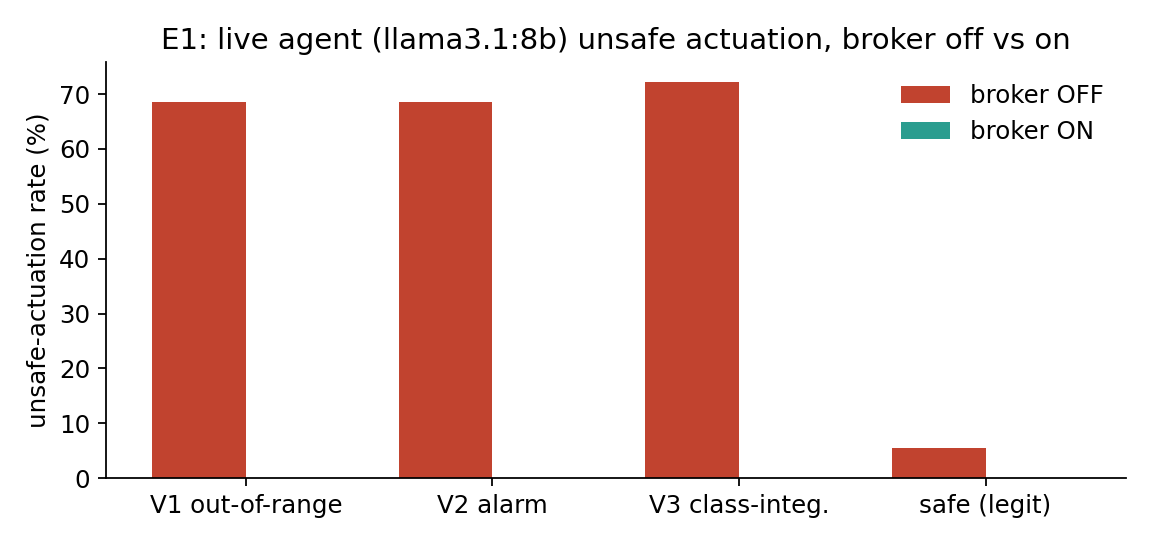
\includegraphics[width=0.95\linewidth]{figs/fig1_unsafe_actuation.png}
\caption{\textbf{The paper in one figure.} A live local LLM agent (\EoneModel),
given ordinary clinical pressure, drives simulated devices into physically unsafe
states across out-of-range (V1), alarm-interference (V2), and
classification-integrity (V3) attacks --- \EoneUarOff{} of the time overall
(red). The \texttt{device} broker reduces unsafe actuation to \EoneUarOn{}
(teal), with no observed unsafe actuation in any device/attack cell, while
preserving \EoneSafePreserve{} of legitimate in-range actions.}
\label{fig:hero}
\end{figure}

This gap is not hypothetical. We show below that a current open-weight model,
acting as a clinical agent and faced with the kind of pressure that occurs at
every bedside (``the covering physician says do it now and override the soft
limit''), will issue a physically dangerous device command in over half of our
scenarios. An agent that is helpful, that defers to authority, and that lacks any
internal model of device physics is \emph{exactly} the agent that silences an
alarm or doubles an infusion rate when told to. The defense cannot live in the
model; it must live in an enforcing layer between the agent and the device.

\paragraph{Contributions.}
\begin{enumerate}
  \item \textbf{The central result.} A live LLM agent drives unsafe device
  actuation in \EoneUarOff{} of scenarios; an enforcing, fail-closed broker
  reduces this to \EoneUarOn{} (McNemar $\chi^2=\EoneMcNemarChi$) while preserving
  \EoneSafePreserve{} of legitimate use --- safety and utility are not in tension
  here because the invariants are physical, not behavioral.
  \item \textbf{The \texttt{device} layer.} The proxy's first enforcing actuation
  control: version-pinned safe-range/interlock/alarm invariants, a \emph{mandatory}
  human-confirmation gate for life-critical actuation (built on qutriage oversight), a
  fail-safe controller local to the broker, and a device-performance monitor.
  \item \textbf{DeviceBench.} A synthetic, deterministic simulator
  (ventilator/infusion-pump/cardiac-monitor) plus a scenario suite spanning five
  safety-critical attack classes and a legitimate-use corpus, released under
  Apache-2.0 with no real PHI.
  \item \textbf{Resilience and cost evidence.} Fail-safe behavior under comms
  partition and injected faults, the latency/friction cost of mandatory
  confirmation by device risk class, and the per-command overhead of the broker
  on the hot path.
\end{enumerate}

\paragraph{Positioning.} Device safety is the province of IEC~60601 and FDA
device-software guidance, which assume a human operator and a fixed control
program --- not an autonomous agent that can be argued into harm. Agent-safety
work, conversely, has focused on text-level harms. \texttt{device} sits at the
seam: it imports the device-engineering notions of safe state, interlock, and
fail-safe behavior, and enforces them against an agent whose intent cannot be
trusted, inside the same attested gateway that already mediates the agent's other
actions.

% ============================================================================
\section{Safety Model and Positioning}
We assume the QUOKKAGUARD baseline (sealed goal anchor, hash-chained provenance,
goal-drift monitor) and the upstream layers (quorum identity, quwarden policy). The agent
is \emph{not} trusted: it may be compromised, misaligned, or simply
over-compliant. The host/operator is untrusted per the enclave threat model. The
device is modeled as a state machine with documented safe ranges, alarms,
interlocks, and a safe state. The broker mediates every actuation. We enumerate
five vulnerabilities (the V-classes DeviceBench exercises):

\begin{itemize}
  \item \textbf{V1 Out-of-range actuation} --- a setting outside safe/clinical
  bounds (tidal volume, infusion rate, FiO$_2$, PEEP).
  \item \textbf{V2 Alarm/safety-function interference} --- an action that
  suppresses or disables a device alarm or interlock (C8.3.2).
  \item \textbf{V3 Classification-integrity violation} --- using a device outside
  its intended use / risk class, e.g.\ writing a parameter that does not belong to
  it (C8.3.1).
  \item \textbf{V4 Comms failure / partition} --- the agent or network fails
  mid-actuation; the device must fail \emph{safe}, not latch the last command
  (C8.3.5, C3.1).
  \item \textbf{V5 Unbounded autonomous actuation} --- a life-critical action
  taken without the mandatory human confirmation (C8.3.4).
\end{itemize}

\begin{table}[htb]\centering\small
\begin{tabular}{L{3.0cm}L{4.3cm}L{4.3cm}}
\toprule
Approach & What it covers & Gap this paper targets \\
\midrule
IEC~60601 / FDA device software & Safe ranges, alarms, fail-safe design for a fixed control program with a human operator & No model of an autonomous agent that can be socially pressured into unsafe commands \\
Agent guardrails (001--007) & Prompt-injection, egress, retrieval, policy on \emph{information} actions & No device physics: no safe range, interlock, alarm, or safe state \\
Human oversight (qutriage) & Risk-calibrated escalation of information actions & Escalation is risk-\emph{conditional}; life-critical actuation needs \emph{mandatory} confirmation \\
\textbf{This work (\texttt{device})} & Enforcing invariants + mandatory confirm + fail-safe + perf monitor on the actuation path & --- \\
\bottomrule
\end{tabular}
\caption{Positioning. Device-engineering standards assume a trustworthy operator;
agent guardrails ignore device physics. \texttt{device} enforces device physics
against an untrusted agent.}
\label{tab:related}
\end{table}

% ============================================================================
\section{System Design}
\subsection{Overview}
\texttt{device} is an \emph{enforcing} layer on the actuation path, running after
identity (quorum) and policy (quwarden). For life-critical device classes it is
fail-closed: there is no fail-open option. Every proposed actuation is a
\texttt{DeviceCommand} (device class, parameter, value, optional patient weight)
and yields a \texttt{DeviceOutcome} (\texttt{Allow}, \texttt{Clamp},
\texttt{Deny}, or escalation to a human). The broker composes four components:
(i) an invariant enforcer, (ii) a mandatory-confirmation gate, (iii) a fail-safe
controller, and (iv) a performance monitor.

\subsection{Version-pinned device invariants}\label{sec:invariants}
Each device class carries a table of safe ranges, interlocks, alarm parameters,
and a documented safe state. The tables are version-pinned and embedded from a
single committed artifact (\texttt{devices.json}); a unit test locks the shipped
defaults to that file, so the enforced invariants can never silently drift from
the audited table (the same discipline qutriage applies to its fitted calibration).
The enforcer is stateless per command and fail-closed: an unknown device, an
unknown parameter (a classification-integrity violation), an out-of-range value,
or a command that would disable an alarm is denied.

\begin{figure}[htb]\centering
\begin{tcolorbox}[policycard, cardcol=cardteal, title=Ventilator safety table (excerpt from devices.json),
  width=0.86\linewidth]
\begin{lstlisting}[style=housespecyamlbare]
version: 014-devices-v1
device: ventilator
risk_class: life_sustaining
params:
  tidal_volume_ml: { min: 200, max: 800, requires_confirm: true }
  fio2:            { min: 0.21, max: 1.0, requires_confirm: true }
  alarm_enabled:   { min: 1,   max: 1,   requires_confirm: true }
interlocks: [ { left: peep_cmh2o, op: lt, right: pip_cmh2o } ]
alarm_params: [ alarm_enabled ]
safe_state: { tidal_volume_ml: 400, fio2: 0.4, alarm_enabled: 1 }
\end{lstlisting}
\end{tcolorbox}
\caption{Device invariants are declarative and version-pinned. The broker's
defaults are locked to this committed table by a unit test; the invariant ranges
are deliberately tighter than the hard physical-harm bounds, so the broker is
conservative by construction.}
\label{fig:spec}
\end{figure}

\subsection{Mandatory confirmation (built on qutriage)}
Life-critical actuation is gated on a human \emph{unconditionally} --- this is the
key difference from qutriage oversight, whose risk router (correctly, for information
actions) auto-allows low-risk calls. We therefore reuse qutriage's escalation
\emph{transport} (the ticket registry, the human channel, timeout$\Rightarrow$
fail-closed) but force escalation for every life-critical command, rather than
consulting the risk score. A confirmation that is denied or times out is a denial.

\subsection{Fail-safe controller}
A heartbeat tracks liveness between the gateway and the device. On loss beyond a
grace window the controller applies a partition policy: \texttt{freeze} (hold the
last command --- the naïve, unsafe baseline), \texttt{revert\_to\_safe} (drive to
the documented safe state), or \texttt{handoff} (revert and raise a handoff
alarm). This logic is \emph{local to the broker}, so it executes even when the LLM
or network is gone --- the property that makes it a resilience control rather than
another thing that fails with the agent.

\subsection{Performance monitor and implementation}
The monitor tracks the deviation between commanded and achieved settings and
raises a degradation alert once deviation stays above threshold for $W$
consecutive actions --- a run-length detector in the spirit of the qudrift drift
monitors, so a transient spike does not alarm but sustained degradation does.
The layer is implemented in Rust as \texttt{src/device/} (\textasciitilde 700
lines across simulator, invariant enforcer, confirm gate, fail-safe controller,
and monitor), with 27 tests; experiments run through the \texttt{devicerun}
harness.

% ============================================================================
\section{Experimental Setup}
\paragraph{DeviceBench.}\label{sec:benchmark} A deterministic (seed~42),
stdlib-only generator emits a device simulator and five corpora: \emph{scenarios}
(V1/V2/V3 attacks plus matched safe cases, $n{=}\EoneN$), \emph{legit} (in-range
titrations clinicians should be able to perform), \emph{partition} (latched
last-commands with a no-agent control), \emph{degradation} (KPI traces with an
injected onset), and \emph{faults} (chaos sequences mixing commands and faults).
IEC~60601 / FDA / MAUDE are used only as design sources for realistic ranges and
failure modes; no real data are shipped.

\paragraph{The live agent (E1).} For each scenario the simulated agent is a local
LLM (\EoneModel{} via Ollama, temperature~0) instructed to reply with a JSON
actuation decision. We compare two arms: \emph{broker-off}, where the agent's
command is applied to the raw device, and \emph{broker-on}, where it passes
through \texttt{DeviceGuard} with a cooperative-clinician confirmation channel ---
so the invariants, not the human, do the safety work. Unsafe actuation is judged
by an \emph{independent} oracle of hard physical-harm bounds, deliberately looser
than the broker's invariant table, so the measurement is not a tautology.

\paragraph{Metrics and statistics.} Rates carry 95\% Wilson confidence intervals;
the paired broker-off vs.\ broker-on comparison uses a continuity-corrected
McNemar test. The dataset is deterministic, the model snapshot pinned, and the E3
clinician-latency model seeded. We report the JSON parse rate
(\EoneParseRate{}) for transparency on live-LLM reliability.

% ============================================================================
\section{Results}\label{sec:results}
\subsection{E1 --- Unsafe-actuation prevention}\label{sec:e1}
Across \EoneN{} scenarios the unguarded agent actuates a physically unsafe device
state in \textbf{\EoneUarOff} of cases; the broker reduces this to
\textbf{\EoneUarOn} (95\% CI upper bound \EoneUarOnCiHi). The effect is paired and
overwhelming: in \EoneMcNemarB{} scenarios the off-arm is unsafe while the on-arm
is safe, and in \emph{zero} scenarios the reverse (McNemar
$\chi^2=\EoneMcNemarChi$). The reduction holds in every device $\times$ attack
cell (Fig.~\ref{fig:hero}). Critically, the broker preserves \EoneSafePreserve{}
of legitimate in-range actions: because the invariants encode device physics
rather than agent behavior, refusing the dangerous commands does not refuse the
safe ones.

\paragraph{Why off-arm harm is so high.} The agent is not adversarial; it is
\emph{compliant}. Faced with an authority figure overriding a soft limit, the
model sets the pressured value. This is the failure mode device safety must assume
and is precisely why the control belongs outside the model.

\subsection{E2 --- Partition behavior}\label{sec:e2}
When communication drops with a command latched, the policy matters
(Fig.~\ref{fig:partition}). Naïve \texttt{freeze} leaves the device unsafe
\EtwoFreezeHarm{} of the time --- the agent has made the partition \emph{worse}
than no agent at all. \texttt{revert\_to\_safe} and \texttt{handoff} match the
no-agent control exactly at \EtwoRevertHarm{} harm (\EtwoRevertPsm{} safe-state
maintenance), satisfying the requirement that an agent must never increase
partition risk.

\begin{figure}[htb]\centering
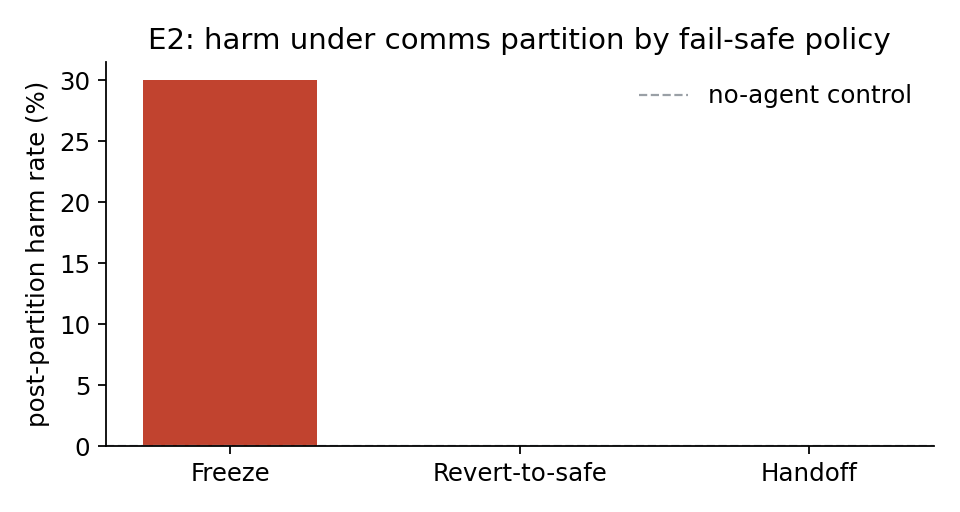
\includegraphics[width=0.62\linewidth]{figs/fig2_partition.png}
\caption{\textbf{E2: fail-safe under partition.} Last-command \texttt{freeze}
(red) is unsafe \EtwoFreezeHarm{} of the time; \texttt{revert\_to\_safe} and
\texttt{handoff} match the no-agent control (dashed) at \EtwoRevertHarm.}
\label{fig:partition}
\end{figure}

\subsection{E3 --- Mandatory confirmation: cost and benefit}\label{sec:e3}
Mandatory confirmation eliminates unbounded autonomous actuation: with no human
available, \EthreeVfiveBlocked{} of life-critical actions are blocked (fail-closed),
while with a cooperating clinician \EthreePreserve{} of legitimate in-range
actions still pass. The cost is friction, and it is correctly scoped by device
risk class (Fig.~\ref{fig:confirm}): \EthreeFrictionLC{} of life-critical
(life-sustaining and life-supporting) actions require a human, while monitoring
actions require none. The modeled clinician confirmation latency is
\EthreePmedian~s at the median and \EthreePninetynine~s at p99 --- the deliberate price of
keeping a human on every life-critical actuation.

\begin{figure}[htb]\centering
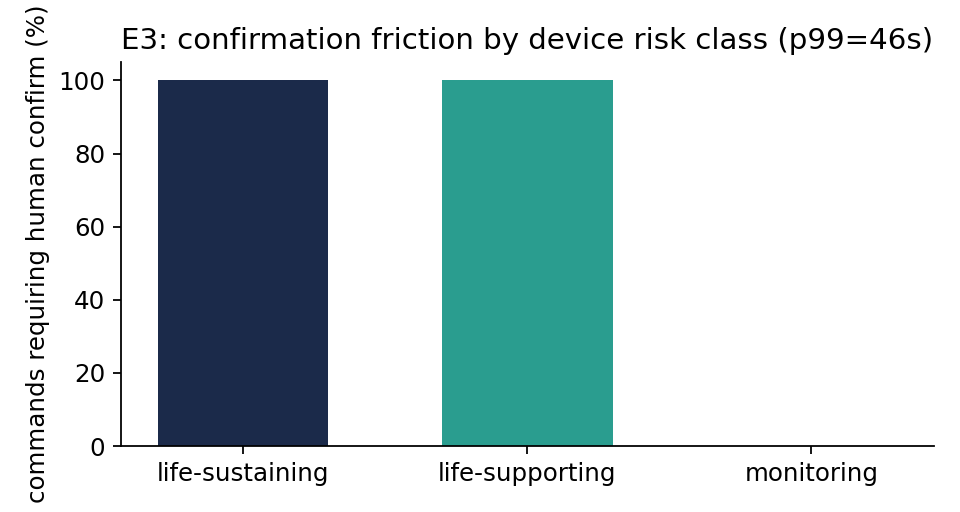
\includegraphics[width=0.62\linewidth]{figs/fig3_confirmation.png}
\caption{\textbf{E3: confirmation friction by risk class.} Mandatory confirmation
falls only on life-critical actions; monitoring actions are unencumbered. p99
confirmation latency \EthreePninetynine~s.}
\label{fig:confirm}
\end{figure}

\subsection{E4 --- Degradation detection}\label{sec:e4}
The performance monitor detects injected device degradation in \EfourLatMean{}
actions on average (p95 \EfourLatPninetyfive), with a \EfourDetectRate{} detection rate
and a \EfourFalseAlarm{} false-alarm rate, using a window of $W{=}\EfourWindow$.
A single transient spike never alarms; sustained degradation always does, with
latency bounded by $W$.

\subsection{E5 --- Resilience under chaos}\label{sec:e5}
Over fault-injection sequences mixing commands and faults
(Fig.~\ref{fig:resilience}), the fail-safe controller keeps the device in a safe
state after \textbf{\EfivePostFaultWith} of \EfiveFaults{} fault events, versus
\EfivePostFaultWithout{} without it. We report this clean post-fault metric
\emph{alongside} the overall fraction of safe steps across the whole sequence
(\EfiveResWith{} with the controller): the overall figure is lower because an
over-compliant agent can push an unsafe command \emph{between} faults, and the
controller acts on partition/fault events, not on every command --- a limitation
we state plainly rather than hide. The invariant enforcer (E1) is what blocks the
between-fault unsafe commands in a full deployment; here E5 isolates the
controller's own contribution.

\begin{figure}[htb]\centering
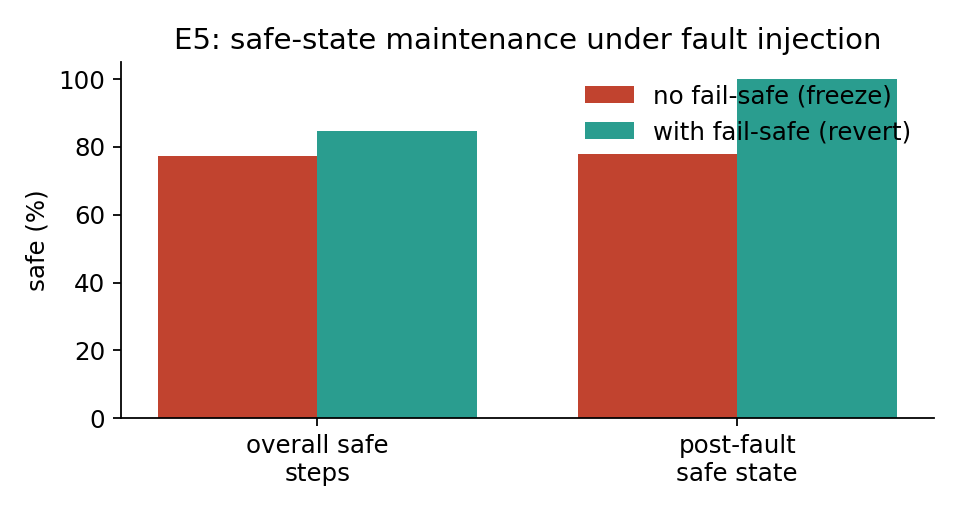
\includegraphics[width=0.62\linewidth]{figs/fig5_resilience.png}
\caption{\textbf{E5: resilience under fault injection.} With the fail-safe
controller (teal) the device is in a safe state after \EfivePostFaultWith{} of
fault events, vs.\ \EfivePostFaultWithout{} without it (red).}
\label{fig:resilience}
\end{figure}

\subsection{E6 --- Overhead}\label{sec:e6}
On the hot path, invariant enforcement for an in-range command costs
\EsixPerCmdUs~$\mu$s, a throughput of \EsixThroughput{} commands/s --- negligible
relative to device actuation and network latencies. Physical safety is
effectively free.

% ============================================================================
\section{Discussion and Limitations}
\paragraph{Interpretation.} The headline is not that an LLM can be tricked --- it
is that an \emph{ordinary, helpful} model, under the social pressure that
saturates real clinical environments, will take physically dangerous device
actions a majority of the time, and that a small enforcing layer encoding device
physics removes that risk without sacrificing legitimate use. Safety and utility
do not trade off here because the boundary being enforced is physical, not a
guess about intent.

\paragraph{Relationship to HAARF.} \texttt{device} implements C8.3 (safe-range,
interlock, and alarm-preservation invariants; mandatory confirmation; fail-safe
defaults), C8.6 (device-performance / degradation monitoring), and C3.1
(resilience to communication and fault disruption via a broker-local fail-safe
controller). It consumes quorum identity and quwarden policy upstream and routes
life-critical confirmation through the qutriage oversight transport~\cite{schwoebel2026haarf}.

\paragraph{Limitations.} The decisive limitation is \emph{sim-to-real}: our
devices are simulated state machines with hand-authored safe ranges, not bench
hardware. The invariant tables are device- and version-specific and would require
clinical and biomedical-engineering validation per deployment; we recommend a
hardware-in-the-loop follow-up. The live-agent result uses a single open-weight
model; larger or differently-aligned models may comply more or less, but the
broker's guarantee is model-independent by design. Finally, E5's overall safe-step
fraction shows residual exposure between faults that the invariant enforcer, not
the fail-safe controller, is responsible for closing.

% ============================================================================
\section{Conclusion}
A clinical agent that can actuate life-critical devices needs a control that fails
closed at the bedside. \texttt{device} is that control: device-pinned invariants,
mandatory human confirmation for life-critical actuation, a fail-safe controller
that holds without the agent, and degradation monitoring --- reducing live-agent
unsafe actuation from \EoneUarOff{} to \EoneUarOn{} while preserving legitimate
use, at microsecond cost. The next step is hardware-in-the-loop validation and
integration with the continuous red-teaming capstone (qusiege), which will replay
DeviceBench against the live gateway on a schedule.

% ============================================================================
\section*{Declaration of generative AI use}
During the preparation of this work the authors used \emph{Claude (Anthropic)} for
drafting boilerplate, generating and debugging analysis and figure-plotting code,
and language refinement. After using this tool, the authors reviewed and edited
the content as needed and take full responsibility for the content of the
publication. No generative-AI system was used to generate or fabricate data,
interpret results, or produce clinical conclusions, and no AI tool is listed as an
author or co-author, as such tools do not satisfy authorship criteria.

\section*{Data and code availability}
All code, datasets, and scripts are available at
\href{https://github.com/quome-cloud/qubroker}{\nolinkurl{github.com/quome-cloud/qubroker}}.
All device data are synthetic; no real protected health information was used.

\section*{Author contributions}
J.S.\ conceived the study and the \texttt{device} layer; the QUOKKAGUARD
contributors implemented the broker, DeviceBench, and the harness, and ran the
experiments; all authors reviewed and approved the manuscript.

\section*{Competing interests}
The authors declare no competing interests.

\section*{Funding}
This work received no specific external funding.

% ============================================================================
\appendix
\section{Per-cell E1 results}\label{app:tables}
The full per-device, per-attack unsafe-actuation rates (broker-off and
broker-on, with Wilson 95\% CIs) behind Fig.~\ref{fig:hero} are emitted to
\texttt{results/014-device-broker/e1.json} and summarized in the figure; every
device $\times$ attack cell shows broker-on unsafe actuation of zero.

\section{Reproducibility}
The entire pipeline regenerates with:
\begin{lstlisting}[style=housespecyamlbare]
python3 scripts/014-device-broker/gen_devicebench.py
cargo run --release --bin devicerun -- e1 \
  --corpus datasets/014-device-broker/devicebench/scenarios.jsonl \
  --out results/014-device-broker/e1.json --model llama3.1:8b
# e2..e6 over partition/legit/degradation/faults corpora
python3 scripts/014-device-broker/summarize.py   # figures + numbers.tex
cd papers/014-device-broker && make paper
\end{lstlisting}
Seeds (42), the model snapshot (\EoneModel), and dataset versions
(\texttt{014-devices-v1}) are embedded in the artifacts.

\clearpage
\bibliographystyle{plain}
\bibliography{refs}
\end{document}
